\documentclass[12pt,a4paper]{article}
%\usepackage[in]{fullpage}
\usepackage[utf8x]{inputenc}
\usepackage{cite}
%\usepackage{listings}
\usepackage[usenames]{xcolor}
\usepackage{graphicx}
\usepackage{hyperref}
\usepackage{float} %for H positioning

%\lstset{ %
%  basicstyle=\footnotesize,        % the size of the fonts that are used for the code
%  breakatwhitespace=true,          % sets if automatic breaks should only happen at whitespace
%  breaklines=true,                 % sets automatic line breaking
%  commentstyle=\color{gray},    % comment style
%  keepspaces=true,                 % keeps spaces in text, useful for keeping indentation of code (possibly needs columns=flexible)
%  language=bash                 % the language of the code
%}

%opening
\title{EVR Tutorials}
%\author{Sašo Skube, PSI}
\date{}

\begin{document}

\maketitle

\tableofcontents
\newpage

\section{Introduction}
A timing system consists of an event generator (EVG), a series of event receivers (EVR), software controlling them and a timing network. EVG generates a series of events, which are delivered to EVRs through a timing network. An EVR is then configured to respond to specific events in various ways, including processing EPICS records and generating pulses, synchronized clock or custom signals on its outputs.
This document contains step-by-step instructions to configuring some of the basic functionalities of the event receiver. A detailed EVR manual is available in~\cite{evr_manual}.

\section{Quick start}\label{sec:Quick start}
To set up a timing system we need a VME crate, a Single Board Computer (SBC) and an EVR. A VME crate has a number of slots where SBC, EVR and other components can be inserted. Slot numbering should be checked with the VME crate documentation. The tutorials in this document are written for the following setup:
\begin{itemize}
	\item a VME64x IFC 1210 Single Board Computer inserted into VME crate slot 1 (how to set up IFC 1210~\cite{ifc}),
	\item VME-EVR-230RF event receiver inserted in slot 2,
	\item the EVR connected to the timing network through an optical cable.
\end{itemize}

To set up an IOC application for EVR we need to set up a startup script and a substitution file. Suitable ones are available in \texttt{\$(TEMPLATES)/EVR} folder. The \texttt{\$(TEMPLATES)} variable is set automatically by the system like so: 
\begin{verbatim}
$(TEMPLATES) = $INSTBASE/iocBoot/templates
\end{verbatim}
Here are a few examples of the \texttt{\$(TEMPLATES)} variable:
\begin{itemize}
	\item \texttt{/fin/devl/iocBoot/templates}
	\item \texttt{/work/iocBoot/templates}
	\item \texttt{/trfcb/work/iocBoot/templates}
\end{itemize}
The following steps demonstrate how to prepare a SWIT compatible IOC application that utilizes EVR:
\begin{enumerate}

	\item Create a project folder, eg. \texttt{MTEST-VME-EVRTEST} and a sub-folder named \texttt{cfg} in your project folder: \texttt{MTEST-VME-EVRTEST/cfg/}
\begin{verbatim}
	mkdir MTEST-VME-EVRTEST
	cd MTEST-VME-EVRTEST
	mkdir cfg
\end{verbatim}

	\item Create a substitution file for your project (can be empty), named \texttt{MTEST-VME-EVRTEST\_main.subs} using the following command: 
\begin{verbatim}
	touch MTEST-VME-EVRTEST_main.subs
\end{verbatim}	
	This substitution file can be used to load custom templates. % that are not directly connected to the basic functionality of the EVR.
	
	\item Copy the startup script \newline \texttt{\$(TEMPLATES)/EVR/example.startup} to your project and rename it to \texttt{MTEST-VME-EVRTEST\_startup.script} using the following command in your project folder:
\begin{verbatim}
	cp $INSTBASE/iocBoot/templates/EVR/example.startup 
	    MTEST-VME-EVRTEST_startup.script
\end{verbatim}

	The startup script should look similar to:
\begin{verbatim}
	## System configuration
	epicsEnvSet SYS MTEST-VME-EVRTEST
	
	### EVR configuration
	#epicsEnvSet EVR EVR0 ##EVR name (default: EVR0)
	#epicsEnvSet EVR_SLOT 3 ##EVR SLOT (default: 2)
	#epicsEnvSet EVR_MEMOFFSET 0xfffff ## A24 base address
	#                                     (default: 0x3000000)
	#epicsEvnSet EVR_IRQLINE 0xff ## IRQ level (default: 0x5)
	#epicsEvnSet EVR_IRQVECT 0xff ## IRQ vector (default: 0x26)
	
	< $(TEMPLATES)/EVR/EVR_VME.startup
	
	## END OF EVR configuration
\end{verbatim}

The configurable variables in the startup script are:
\begin{itemize}
%	\item 
%		\texttt{TEMPLATES} is the location of the template files. It is automatically set based on \texttt{INSTBASE}.
	\item
		\texttt{SYS} is the system name. \textbf{This variable is mandatory.}
	\item 
		\texttt{EVR} is the event receiver name. If the variable is not defined in the startup script, it defaults to \texttt{EVR0}.
	\item 
		\texttt{EVR\_SLOT} is the VME crate slot where EVR is inserted. If the variable is not defined in the startup script, it defaults to \texttt{2}.
	\item 
		The the base A24 address (\texttt{EVR\_MEMOFFSET}), interrupt level (\texttt{EVR\_IRQLINE}) and interrupt vector (\texttt{EVR\_IRQVECT}) variables configure the interaction between the SBC and the EVR. The details are out of scope of this document. If a variable is not defined in the startup script, it gets set to its default value.
\end{itemize}
Using the above startup script, the system name is set to \textit{MTEST-VME-EVRTEST}, and the event receiver named \textit{EVR0} is placed in the physical slot 2 of the VME crate. It uses default A24 address and interrupt configuration.

Line \texttt{$<$ \$(TEMPLATES)/EVR\_VME.startup} includes a generic EVR startup script, and must not be changed by the user.

	\item Copy the substitution file \texttt{\$INSTBASE/iocBoot/templates/EVR/EVR.subs} to \texttt{MTEST-VME-EVRTEST/cfg/EVR.subs}. This substitution file can always be used as a starting point for new applications. Use the following command in your project folder: 
\begin{verbatim}
	cp $INSTBASE/iocBoot/templates/EVR/EVR.subs cfg/
\end{verbatim}
The macro definitions in the substitution file are used to configure the EVR. All the available macros are already present in the substitution file and set to their default values, so the user can simply change the desired values. Detailed description of the substitution file is available in the EVR manual~\cite{evr_manual}.
\end{enumerate}



%\paragraph{Command summary} for creating a new IOC application:
%\begin{verbatim}
%	mkdir MTEST-VME-EVRTEST
%	cd MTEST-VME-EVRTEST
%	mkdir cfg
%	cp /fin/devl/iocBoot/templates/EVR/example.startup 
%	    MTEST-VME-EVRTEST_startup.script
%	cp /fin/devl/iocBoot/templates/EVR/EVR.subs cfg/
%\end{verbatim}

\section{Generate a pulse upon receiving an event}
EVR has a number of pulsers available and each of them can generate a pulse upon receiving an event. The pulse can then be outputted through desired EVR outputs. 

This tutorial demonstrates how to configure an EVR to generate a 80 ns wide pulse, 40 ns after each reception of event 4, as seen in Figure~\ref{fig:pulser_signal}. 
\begin{figure}[H]
	\centering
	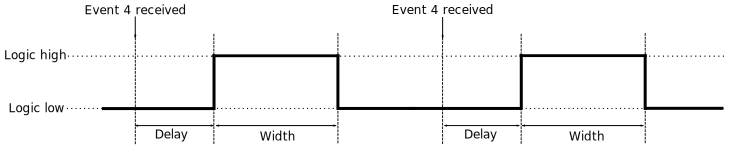
\includegraphics[width=\columnwidth]{./img/pulserSignal}
	\caption{An example of a pulse generated after the reception of the event 4.}
	\label{fig:pulser_signal}
\end{figure}
The pulse in this tutorial is generated using pulser 3 and outputted through the front panel TTL output 0 (FrontOut0), as seen in Figure~\ref{fig:pulser}. 
%In order to achieve this, pulser 3 delay and width parameters are configured by setting macro value of \texttt{Pul3-Delay-SP} to 40 and of \texttt{Pul3-Width-SP} to 80. Then the value of the output source macro \texttt{FrontOut0-Src-SP} is set to 3, which configures the front panel output 0 (FrontOut0) to use pulser 3 as its source. Finally, pulser 3 is set to trigger on event 4 by setting macro value \texttt{EVT} to 4. 

\begin{figure}[H]
	\centering
	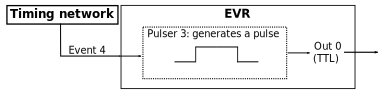
\includegraphics[]{./img/pulser}
	\caption{Use pulser 3 to generate a pulse upon reception of the event 4. The pulse is outputted through front panel TTL output 0.}
	\label{fig:pulser}
\end{figure}

\subsection{Instructions}
\begin{enumerate}
	\item If starting a new IOC application, consult the quick start in Section~\ref{sec:Quick start}.

	\item Set the macro values in the substitution file (\texttt{MTEST-VME-EVRTEST/cfg/EVR.subs}) according to this snippet (explained in~\ref{sec:explain_pulser}):
\begin{verbatim}
	file "$(TEMPLATE_DIR)/evr-vmerf230.template"
	{
	  {
	    ...
	    Pul3-Delay-SP=40,
	    Pul3-Width-SP=80,
	    ...
	    FrontOut0-Src-SP=3,
	    ...
	  }
	}

	file "$(TEMPLATE_DIR)/evr-pulserMap.template"{
	pattern { PID   F,       EVT, ID}
	        ...
	        { 3,    Trig,    4,   0 }
	        ...
	}
\end{verbatim}
	The above macro substitution of the \texttt{evr-vmerf230.template} sets the values of the following records:
	\begin{itemize}
	\item \texttt{MTEST-VME-EVRTEST-EVR0:Pul3-Delay-SP}
	\item \texttt{MTEST-VME-EVRTEST-EVR0:Pul3-Width-SP}
	\item \texttt{MTEST-VME-EVRTEST-EVR0:FrontOut0-Src-SP}
	\end{itemize}
	The above macro substitution of the \texttt{evr-pulserMap.template} creates a record named \texttt{MTEST-VME-EVRTEST-EVR0:Pul\$(PID)-Evt-\$(F)\$(ID)-SP}.
	\item Optionally, you can remove all the macros whose values you did not change. 
	\item Install the prepared IOC by running command \texttt{swit -V} from your project folder \textit{MTEST-VME-EVRTEST}.
\end{enumerate}
\subsection{Substitution snippet explanation:}\label{sec:explain_pulser}

First we set up the pulse generator 3 (Pul3):
\begin{itemize}
	\item \texttt{Pul3-Delay-SP}=40: Set the delay between the reception of the event and the start of the pulse (pulse rising edge) for pulser 3 to 40 ns. 
	\item \texttt{Pul3-Width-SP}=80: Set the pulse width (time between the pulse rising and falling edge) for pulser 3 to 80 ns.
\end{itemize}

Then the value of the output source macro \texttt{FrontOut0-Src-SP} is set to 3, which configures the front panel output 0 (FrontOut0) to use pulser 3 as its source. Macro values 0-15 correspond to pulsers 0-15. A complete list of available values can be found in the EVR manual~\cite{evr_manual}.

Finally, the Pulser 3 is set to trigger on reception of the event 4:
\begin{itemize}
	\item \texttt{PID}: Select Pulser 3
	\item \texttt{F}: Select the \textit{Trigger} function of the pulser
	\item \texttt{EVT}: Map Pulser 3 Trig function to event 4
	\item \texttt{ID}: Unique ID for each PID-F combination.
\end{itemize}

In order to use different pulser simply change the pulser number, eg. using \texttt{Pul5-Delay-SP} instead of \texttt{Pul3-Delay-SP} sets the delay of pulser 5 instead of pulser 3.
Similar is for outputs, eg. using \texttt{FrontOut1-Src-SP} instead of \texttt{FrontOut0-Src-SP} sets the output source signal of front panel output 1 instead of front panel output 0. In order to set a different event mapped to Pulser 3 Trig function, simply set a new value of the record \texttt{MTEST-VME-EVRTEST-EVR0:Pul3-Evt-Trig0-SP}. To disable the mapping, set the record value to \texttt{0}.

\section{Trigger an EPICS event upon receiving an event from the timing system}
Using the macros in the substitution file it is possible to configure triggering of the EPICS events. Each event from the timing system can be configured to trigger an EPICS event.

This tutorial demonstrates how to trigger an EPICS event number 1 upon reception of event 1 from the timing system.

\subsection{Instructions}
\begin{enumerate}
	\item If starting a new IOC application, consult the quick start in Section~\ref{sec:Quick start}.
	
	\item Set the macro values in the substitution file (\texttt{MTEST-VME-EVRTEST/cfg/EVR.subs}) according to this snippet (explained in~\ref{sec:explain_event}):
\begin{verbatim}
	file "$(TEMPLATE_DIR)/evr-softEvent.template"{
	pattern { EVT,    CODE }
	        { "1",    "1"}
	        ...
	}
\end{verbatim}
	\item Optionally, you can remove all the macros whose values you did not change. 

	\item Install the prepared IOC by running command \texttt{swit -V} from your project folder \textit{MTEST-VME-EVRTEST}.
\end{enumerate}

\subsection{Substitution snippet explanation:}\label{sec:explain_event}
An EPICS event 1 (\texttt{CODE=1}) is triggered upon reception of the event a (\texttt{EVT=1}) from the timing system.
It is suggested that macros \texttt{EVT} and \texttt{CODE} are set to the same value for simplicity, all-though this is not mandatory.

%In addition to triggering an EPICS event, a counter is increased. The counter is a calc record, that counts how many times the event was received from the timing system. Its name is in form of \texttt{\$(SYS)-\$(EVR):Event-\$(EVT)-Cnt-I}, where \texttt{\$(SYS)} represents the system name, \texttt{\$(EVR)} represents the event receiver name (eg. EVR0) and \texttt{\$(EVT)} is the event from the timing network. In this example the full \textbf{name of the counter record is} \texttt{MTEST-VME-EVRTEST-EVR0:Event-1-Cnt-I}.

\section{Generate a clock signal}

Event receivers have synchronized event clock across the timing system (the same phase and frequency). The event clock can be prescaled and mapped to the EVR output. The minimum prescale factor is 2, so a clock signal with the same phase and frequency as the event clock cannot be generated this way (Section~\ref{sec:generate_event_clock} describes how to generate the event clock).

This tutorial demonstrates how to configure the prescaler 0 (PS0) to divide the event clock frequency by 2, and output it through the front panel output 1 (FrontOut1), as seen in Figure~\ref{fig:prescaler}. 
%This can be achieved by setting the prescaler macro \texttt{PS0-Div-SP} to 2, and the output source macro \texttt{FrontOut1-Src-SP} to 40. The latter configures the front panel output 1 (FrontOut1) to use prescaler 0 as its source.

\begin{figure}[H]
	\centering
	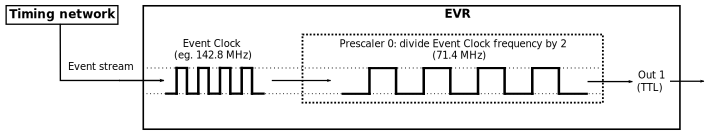
\includegraphics[width=\columnwidth]{./img/prescaler}
	\caption{An example clock signal generation}
	\label{fig:prescaler}
\end{figure}

\subsection{Instructions}
\begin{enumerate}
	\item If starting a new IOC application, consult the quick start in Section~\ref{sec:Quick start}.

	\item Set the macro values in the substitution file (\texttt{MTEST-VME-EVRTEST/cfg/EVR.subs}) according to this snippet (explained in~\ref{sec:explain_clock}):
\begin{verbatim}
	file "$(TEMPLATE_DIR)/evr-vmerf230.template"
	{
	  {
	    ...
	    PS0-Div-SP=2,
	    ...
	    FrontOut1-Src-SP=40,
		    ...
	  }
	}
\end{verbatim}
	The above macro substitution of the \texttt{evr-vmerf230.template} sets the values of the following records:
	\begin{itemize}
		\item \texttt{MTEST-VME-EVRTEST-EVR0:PS0-Div-SP}
		\item \texttt{MTEST-VME-EVRTEST-EVR0:FrontOut1-Src-SP}
	\end{itemize}
	
	\item Optionally, you can remove all the macros whose values you did not change. 
	\item Install the prepared IOC by running command \texttt{swit -V} from your project folder \textit{MTEST-VME-EVRTEST}.
\end{enumerate}

\subsection{Substitution snippet explanation:}\label{sec:explain_clock}
\begin{itemize}
	\item \texttt{PS0-Div-SP}=2: Set the Prescaler 0 to divide event clock frequency by 2.
	\item \texttt{FrontOut1-Src-SP}=40: Set the source of the Front Panel Output 1 to Prescaler 0. Values 40-42 correspond to prescalers 0-2. A complete list of values is available in the EVR manual~\cite{evr_manual}.
\end{itemize}

In order to use different prescaler, simply change the prescaler number, eg. using \texttt{PS2-Div-SP} instead of \texttt{PS0-Div-SP} sets the divider of prescaler 2 instead of prescaler 0.
Similar is for outputs, eg. using \texttt{FrontOut0-Src-SP} instead of \texttt{FrontOut1-Src-SP} sets the output source signal of front panel output 0 instead of front panel output 1.

\section{Generate the event clock}\label{sec:generate_event_clock}
Signals with frequency greater or equal to the frequency of the event clock can only be generated using the CML outputs. More about the operation of the CML outputs and their modes is available in the EVR manual~\cite{evr_manual}. Note, that not all event receiver form factors have CML outputs. The EVR-VME-230RF form factor has outputs FrontOut4 (CML0), FrontOut5 (CML1) and FrontOut6 (CML2) capable of CML output. This tutorial demonstrates how to configure CML0 output (corresponds to FrontOut4 output) to generate a clock signal, that has the same phase and frequency as the event clock. To achieve this, the FrontOut4 output source is set to \texttt{logic low} and the CML outputs are enabled. This causes the logic low pattern of the CML pulse mode to be continuously outputted. The configurable pattern, as seen in Figure~\ref{fig:gen_evt_clk}, is 20 bits long and is sent out with a bit rate of 20 times the event clock rate. It is configured to replicate the event clock phase and frequency.

\begin{figure}[H]
	\centering
	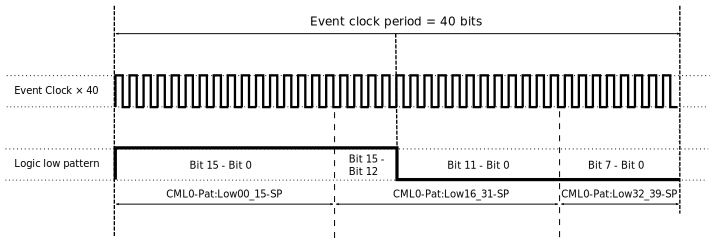
\includegraphics[width=\columnwidth]{./img/gen_evt_clk}
	\caption{Generate the event clock}
	\label{fig:gen_evt_clk}
\end{figure}

\subsection{Instructions}
\begin{enumerate}
	\item If starting a new IOC application, consult the quick start in Section~\ref{sec:Quick start}.
	
	\item Set the macro values in the substitution file (\texttt{MTEST-VME-EVRTEST/cfg/EVR.subs}) according to this snippet (explained in~\ref{sec:explain_cml}):
\begin{verbatim}
	file "$(TEMPLATE_DIR)/evr-vmerf230.template"
	{
	  {
	    ...
	    FrontOut4-Ena-SP=1,
	    FrontOut4-Src-SP=63,
	    CML0-Ena-Sel=1,
	    CML0-Pwr-Sel=1,
	    CML0-Mode-Sel=0,
	    CML0-Pat:Low00_15-SP=0xFFC0,
	    CML0-Pat:Low16_31-SP=0, 
	    ...
	  }
	}
\end{verbatim}
	The above macro substitution of the \texttt{evr-vmerf230.template} sets the values of the following records:
	\begin{itemize}
		\item \texttt{MTEST-VME-EVRTEST-EVR0:FrontOut4-Ena-SP}
		\item \texttt{MTEST-VME-EVRTEST-EVR0:FrontOut4-Src-SP}
		\item \texttt{MTEST-VME-EVRTEST-EVR0:CML0-Ena-Sel}
		\item \texttt{MTEST-VME-EVRTEST-EVR0:CML0-Pwr-Sel}
		\item \texttt{MTEST-VME-EVRTEST-EVR0:CML0-Mode-Sel}
		\item \texttt{MTEST-VME-EVRTEST-EVR0:CML0-Pat:Low00\_15-SP}
		\item \texttt{MTEST-VME-EVRTEST-EVR0:CML0-Pat:Low16\_31-SP}
	\end{itemize}

	\item Optionally, you can remove all the macros whose values you did not change. 
	\item Install the prepared IOC by running command \texttt{swit -V} from your project folder \textit{MTEST-VME-EVRTEST}.
\end{enumerate}

\subsection{Substitution snippet explanation:}\label{sec:explain_cml}
\begin{itemize}
	\item \texttt{FrontOut4-Ena-SP}=1: Enable the front panel output 4.
	\item \texttt{FrontOut4-Src-SP}=63: Set the source of the front panel output 4 to logic low. A complete list of settable values is available in the EVR manual~\cite{evr_manual}.
	\item \texttt{CML0-Ena-Sel}=1: Enable the CML0 output, which corresponds to the front panel output 4.
	\item \texttt{CML0-Pwr-Sel}=1: Power on the CML0 output.
	\item \texttt{CML0-Mode-Sel}=0: Select the pulse mode. Because the output source signal of the front panel output 4 is set to logic low, this mode will continuously output logic low pattern.
	\item \texttt{CML0-Pat:Low00\_15-SP}=0xFFC0: Set logic low pattern bits 0-15. The Figure~\ref{fig:gen_evt_clk} shows that the bits 15-0 must be set as follows: \texttt{1111 1111 1100 0000}, which translates to \texttt{0xFFC0}. Each bit represents $1/20$ of the event clock period.
	\item \texttt{CML0-Pat:Low16\_31-SP}=0: Set signal low pattern bits 16-31, as seen in Figure~\ref{fig:gen_evt_clk}. Note, that only bits 31-28 (top 4 bits) can be used.
\end{itemize}


\section{Output a Distributed Bus bit}
A custom distributed bus (DBus) bit can be outputted through desired EVR outputs. This tutorial demonstrates how to set up the DBus bit 0 as a source of an EVR front panel output 1, as seen in Figure~\ref{fig:dbus}. 
%To achieve this, the front panel output 0 should be mapped to the distributed bus bit (signal) 0. This is configured by setting the value of the output source macro \texttt{FrontOut1-Src-Sp} to 32. Mapping 32 corresponds to the DBus bit 0.

\begin{figure}[H]
	\centering
	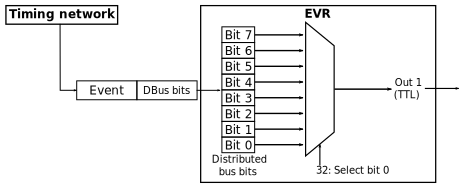
\includegraphics[]{./img/dbus}
	\caption{Send DBus bit 0 to the front panel output 1}
	\label{fig:dbus}
\end{figure}

\subsection{Instructions}
\begin{enumerate}
	\item If starting a new IOC application, consult the quick start in Section~\ref{sec:Quick start}.
	
	\item Set the macro values in the substitution file (\texttt{MTEST-VME-EVRTEST/cfg/EVR.subs}) according to this snippet (explained in~\ref{sec:explain_dbus}):
\begin{verbatim}
	file "$(TEMPLATE_DIR)/evr-vmerf230.template"
	{
	  {
	    ...
	    FrontOut1-Src-SP=32,
	    ...
	  }
	}
\end{verbatim}
	The above macro substitution of the \texttt{evr-vmerf230.template} sets the values of the following record:
	\begin{itemize}
		\item \texttt{MTEST-VME-EVRTEST-EVR0:FrontOut1-Src-SP}
	\end{itemize}

	\item Optionally, you can remove all the macros whose values you did not change. 
	\item Install the prepared IOC by running command \texttt{swit -V} from your project folder \textit{MTEST-VME-EVRTEST}.
\end{enumerate}

\subsection{Substitution snippet explanation:}\label{sec:explain_dbus}
\begin{itemize}
	\item \texttt{FrontOut1-Src-SP}=32: Set the source of the front panel output 1  to DBus bit 0. Values 32-39 correspond to DBus bits 0-7. A complete list of values is available in the EVR manual~\cite{evr_manual}.
\end{itemize}

In order to use different front panel output, simply change the front panel output number, eg. using \texttt{FrontOut0-Src-SP} instead of \texttt{FrontOut1-Src-SP} sets the output source signal of front panel output 0 instead of front panel output 1.

\section{Data buffer}\label{sec:data_buffer}
The timing system supports deterministic data transmission. Data buffer enables the event receivers to accept the transmitted data in a buffer. The data can be written and read from through EPICS records, which access the buffer in the EVR.

When using the EVR as described in Section~\ref{sec:Quick start}, the following data/records are already available:
\begin{itemize}
\item Data regarding the beam synchronous readouts~\cite{bsread}:
	\begin{itemize}
	\item \texttt{\$(SYS)-\$(EVR):BunchIdRx-I}: The pulse ID,
	\item \texttt{\$(SYS)-\$(EVR):BunchIdRx-MASTER-TS-SEC}: Seconds part of the pulse time-stamp,
	\item \texttt{\$(SYS)-\$(EVR):BunchIdRx-MASTER-TS-NSEC}: Nanoseconds part of the pulse time-stamp,
	\end{itemize}
\end{itemize}
where \texttt{\$(SYS)} is the system name (\textit{MTEST-VME-EVRTEST}) and \texttt{\$(EVR)} is the event receiver name (\textit{EVR0}).

\begin{quote}
\textbf{Adding data to the buffer should be coordinated with the entire team. Special care should be taken in order to avoid destroying existing data in the buffer.}
\end{quote}

The following instructions show how to use a combination of analogue in and analogue out records to read and write custom data in the data buffer:
\begin{enumerate}
\item If starting a new IOC application, consult the quick start in Section~\ref{sec:Quick start}.
\item Create a new template file named \texttt{customData.template} with the following content in the project folder \textit{MTEST-VME-EVRTEST}:
	\begin{verbatim}
		record(ao, "$(SYS)-$(EVR):customData$(ID)-SP") {
		  field(DTYP, "regDev")
		  field(OUT, "@EVRDBUFF:$(OFFSET) T=double")
		}
		
		record(ai, "$(SYS):$(EVR)-customData$(ID)-RB") {
		  field(DTYP, "regDev")
		  field(INP, "@EVRDBUFF:$(OFFSET) T=double")
		  field(SCAN, "I/O Intr")
		}
	\end{verbatim}
	The \texttt{\$(SYS)-\$(EVR):customData\$(ID)-SP} record is used to write the data at the specified offset in the data buffer. Once the data is written, it can be read from any EVR in the timing system, which has the counterpart \texttt{\$(SYS):\$(EVR)-customData\$(ID)-RB} record (an analogue in record with the same offset).
	\begin{itemize}
		\item 
			\texttt{\$(SYS)} is the system name, and \texttt{\$(EVR)} is the event receiver name. The \texttt{\$(ID)} is a unique identification of the record.
		\item 
			In order to use records for reading and writing data to the data buffer, device type must be set to \texttt{regDev}~\cite{regDev}.
		\item 
			\texttt{INP} and \texttt{OUT} fields of the record specify the type of the data (\texttt{T=double}), the buffer name and the buffer offset(\texttt{\$(OFFSET)}) to read/write. When using the EVR as described in Section~\ref{sec:Quick start}, the buffer name is always \texttt{EVRDBUFF}. Offset is in range of \texttt{0x04 - 0x7FC} bytes.
		\item 
			When new data is available to read, an interrupt is fired. The \texttt{\$(SYS):\$(EVR)-customData\$(ID)-RB} record gets processed on each interrupt (\texttt{field(SCAN, "I/O Intr")}), thus the record's value is updated with the new data.
	\end{itemize}

\item Add the following to the \texttt{MTEST-VME-EVRTEST\_main.subs} file:
	\begin{verbatim}
	file "customData.template"{
	pattern {  SYS,                    EVR,    ID, OFFSET }
	        { "MTEST-VME-EVRTEST",    "EVR0",  0,  0x50}
	        { "MTEST-VME-EVRTEST",    "EVR0",  1,  0x60}
	}
	\end{verbatim}
	The above substitution creates the following records:
	\begin{itemize}
		\item \texttt{MTEST-VME-EVRTEST:EVR0-customData0-SP}: Used to write a value of type double to buffer offset \texttt{0x50}.
		\item \texttt{MTEST-VME-EVRTEST:EVR0-customData1-SP}: Used to write a value of type double to buffer offset \texttt{0x60}.
		\item \texttt{MTEST-VME-EVRTEST:EVR0-customData0-RB}: Used to read a value of type double from the buffer offset \texttt{0x50}
		\item \texttt{MTEST-VME-EVRTEST:EVR0-customData1-RB}: Used to read a value of type double from the buffer offset \texttt{0x60}
	\end{itemize}
\item Install the prepared IOC by running command \texttt{swit -V} from your project folder \textit{MTEST-VME-EVRTEST}.
\end{enumerate}

\section{GUI}\label{sec:gui} 
There is a caQtDM~\cite{caqtdm} GUI for the Event Receiver available. It can be used to further configure the EVR or simply check the running configuration. The GUI is launched using the following command:

\begin{verbatim}
	start_EVR.sh -s SYS [options]
\end{verbatim}
where the \texttt{SYS} represents a \textbf{mandatory} system name, and \texttt{[options]} are as follows:
\begin{verbatim}
	-r <EVR name> ......... set the event receiver name 
	                        (default:EVR0)
	-f <form factor> ...... choose the event receiver form factor 
	                        (default: VME)
	                        Choices: VME, PCIe
	-h    ................. shows the options and usage
\end{verbatim}


\paragraph{Example 1:} Open the GUI for the EVR-VME-230RF event receiver named \texttt{EVR0}, using system name \texttt{MTEST-VME-EVRTEST}.
\begin{verbatim}
	start_EVR.sh -s MTEST-VME-EVRTEST
\end{verbatim}

\paragraph{Example 2:} Open the GUI for the EVR-VME-230RF event receiver named \texttt{EVR3}, using system name \texttt{MTEST-VME-EVRTEST}.
\begin{verbatim}
	start_EVR.sh -s MTEST-VME-EVRTEST -r EVR3
\end{verbatim}

\paragraph{Example 2:} Open the GUI for the EVR-PCIe-300 event receiver named \texttt{EVR0}, using system name \texttt{MTEST-VME-EVRTEST}.
\begin{verbatim}
	start_EVR.sh -s MTEST-VME-EVRTEST -f PCIe
\end{verbatim}

\paragraph{Example 3:} Shows options and usage.
\begin{verbatim}
	start_EVR.sh -h
\end{verbatim}

\bibliographystyle{plain}
\bibliography{references}

\end{document}
